\documentclass[../master]{subfiles}

%\graphicspath{{../eps/}}

\begin{document}

\chapter{中性子コリメータ}
\section{ビームサイズを制限する必要性}
中性子ビームは可能な限り細いのもが望ましい.
例えば,半径\SI{50}{\milli\metre}の幅を持っている中性子ビームを用いると,
散乱点が$y$軸方向に\SI{100}{\milli\metre}の幅を持つ.
gridの座標を$y = \SI{0}{\milli\metre}$,plateの座標を$y = \SI{140}{\milli\metre}$とし,
ビームの中心が$y = \SI{70}{\milli\metre}$の位置にあるとすると,
中性子ビームは$y = $\SIrange{20}{120}{\milli\metre}の範囲に入射する.
この時$y = \SI{120}{\milli\metre}$の位置で散乱が起きると,
見かけ上の有感領域はgrid方向に\SI{120}{\milli\metre},plate方向に\SI{20}{\milli\metre}となる.
反対に,$y = \SI{20}{\milli\metre}$の位置で散乱が起きると,
見かけ上の有感領域はgrid方向に\SI{20}{\milli\metre},plate方向に\SI{120}{\milli\metre}となる.
しかし,MAIKo TPC は$y$座標をトラックの周囲に発生した電子の読み出し面に到達する時間差を用いて検出しているため,
$y$座標の絶対値を決定することができない.
すると,$y = \SI{120}{\milli\metre}$と$y = \SI{20}{\milli\metre}$のどちらで散乱が起きたのかを区別できない.
どちらの場合でも確実に有感領域中で停止したと保証するためには,
散乱点から$y$軸方向に\SI{\pm20}{\milli\metre}を実質の有感領域としなければならない.

有感領域が小さいと領域外に出ていく$\alpha$粒子の数が増えてしまい,
検出効率が低下する.
そのため,中性子ビームの$y$軸方向のサイズは可能な限り小さいのもが望ましい.
その反面,ビームを補足すると標的で生成された中性子を制限することになるので,
中性子の入射量が低下する.
この2つの効果を考慮して収量が大きくなるビームサイズを決定する.

\section{シミュレーションによるビームサイズの決定}
重照射室内のトリチウムターゲットから中性子は$4\pi$に等方的に放出していると仮定する.
すると,中性子の収量はコリメータの立体角で決定される.
トリチウムターゲットから重照射室の大実験室側の壁までの距離は\SI{1.46e3}{\milli\metre},
壁の厚さは\SI{1e3}{\milli\metre}である.
コリメータの半径を$r$~\si{\milli\metre}とすると,立体角は
$\pi\times r^2/\left(2.46\times10^3\right)^2$となる.
図\ref{fig::alpha_E_dist}のエネルギー分布を仮定して,
$\alpha$粒子の検出効率を求めた.
\SIrange{5}{50}{\milli\metre}でのコリメータの立体角の割合と検出効率を
表\ref{tab::solid_angle_percent}に示す.
検出効率は\SI{10}{\milli\metre}以下ではあまり変化がない.
\SI{5}{\milli\metre}と\SI{10}{\milli\metre}を比較すると,
立体角は4倍\SI{10}{\milli\metre}の方が大きい.
大きな検出効率を持ちつつ立体角が大きい\SI{10}{\milli\metre}のコリメータを用いる.
%コリメータの立体角と検出効率の積が最も大きくなるところが収量が最も大きくなる.
\begin{table}
  \centering
  \caption{コリメータの半径とコリメータの立体角,検出効率.}
  \label{tab::solid_angle_percent}
  \begin{tabular}{ccc}
    \toprule
    コリメータの半径 (\si{\milli\metre}) & 立体角 (\si{\steradian}) & 検出効率 (\si{\percent})\\% & 積\\
    \midrule
     5 & $1.30\times10^{-5}$ & 48.7 \\%& $6.33\times10^{-6}$ \\
    10 & $5.19\times10^{-5}$ & 48.2 \\%& $2.50\times10^{-5}$ \\
    20 & $2.08\times10^{-4}$ & 46.6 \\%& $9.69\times10^{-5}$ \\
    30 & $4.67\times10^{-4}$ & 39.2 \\%& $1.83\times10^{-4}$ \\
    40 & $8.31\times10^{-4}$ & 26.3 \\%& $2.19\times10^{-4}$ \\
    50 & $1.30\times10^{-3}$ & 10.3 \\%& $1.34\times10^{-4}$ \\
    \bottomrule
  \end{tabular}
\end{table}

\section{コリメータの作成}
中性子を遮蔽する材料として,陽子を多く含むポリエチレンや吸収断面積が大きいホウ素が広く用いられている.
ポリエチレンとホウ素入りポリエチレンでの中性子の遮蔽度合いをPHITS (ver.~3.14)~\cite{phits}を用いて計算した.
図\ref{collimator_xy_pos}は\SI{14}{\mega\electronvolt}の中性子がコリメータを通過したときの位置分布である.
2つの中性子の分布に大きな差異は見られない.
図\ref{fig::neutron_energy_dist},\ref{fig::neutron_energy_dist_w_B}はコリメータを通過した後の中性子のエンルギー分布である.
青色のヒストグラムは\SIrange{0}{10}{\milli\metre}の範囲の中性子,
赤色のヒストグラムは\SIrange{10}{55}{\milli\metre}の範囲の中性子のエネルギー分布である.
コリメータの穴の部分に対してポリエチレンまたはホウ素入りポリエチレンの部分は
中性子が遮蔽されいることが分かる.
ポリエチレンとホウ素入りポリエチレンでは同程度にコリメートできているので,
本実験ではコストの面からポリエチレンを用いたコリメータを作成した.
実際に作成したコリメータを図\ref{pic::collimator}に示す.
このコリメータは半径\SI{55}{\milli\metre},高さ\SI{100}{\milli\metre}の円柱の中心に
半径\SI{10}{\milli\metre}の穴を開けた構造になっている.
壁の厚さが\SI{1000}{\milli\metre}であるため,
このコリメータ10 個を中性子の取り出し穴に挿入する.
\begin{figure}
  \centering
  \begin{subfigure}{0.45\columnwidth}
    \centering
    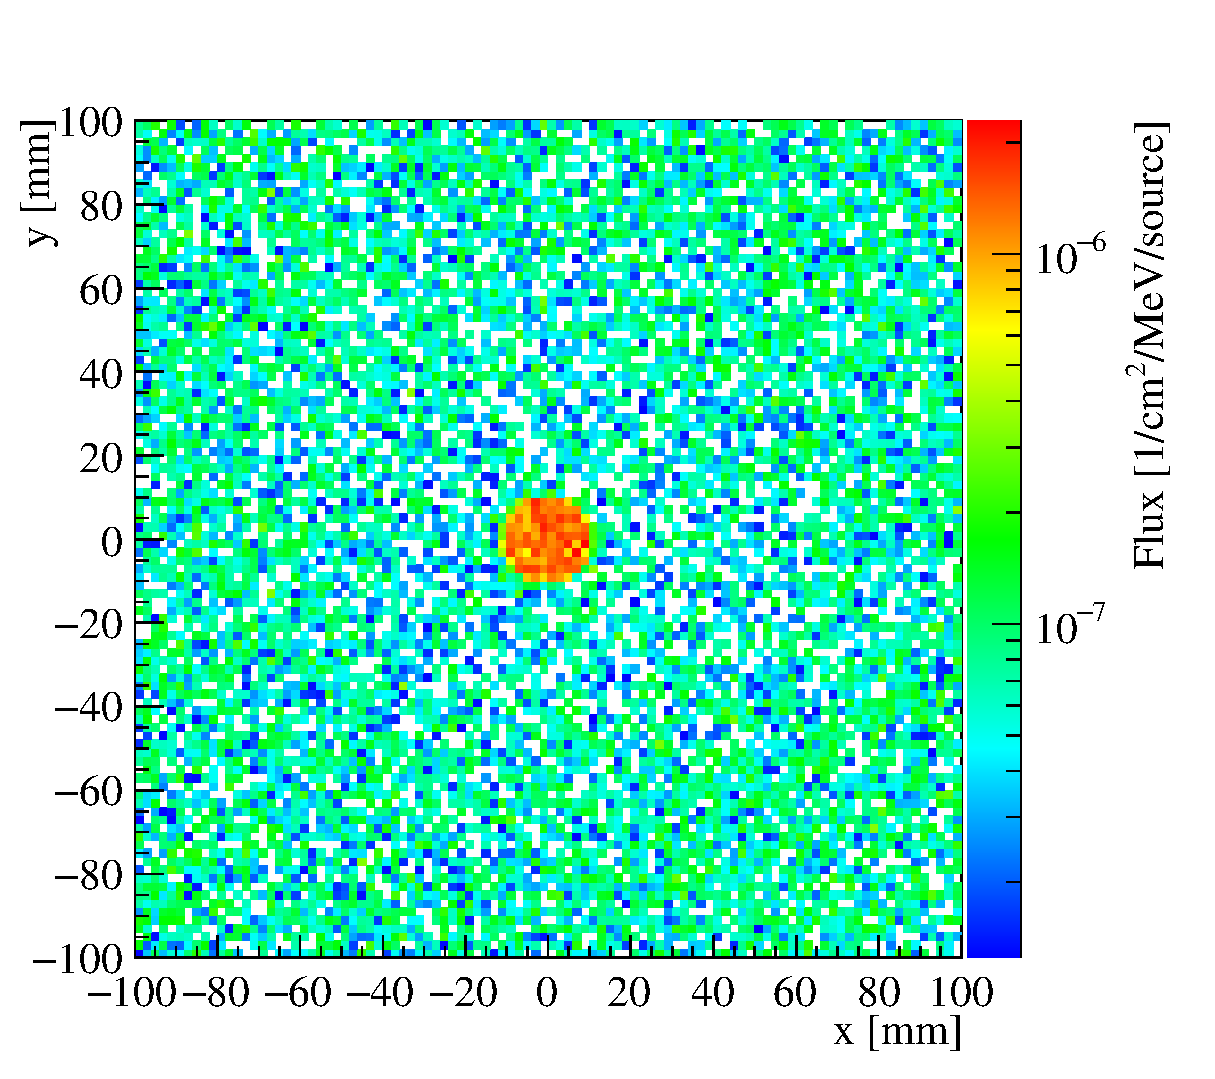
\includegraphics[clip, width=\columnwidth]{cross_xy_f.eps}
    \caption{ポリエチレンの場合.}
  \end{subfigure}
  \begin{subfigure}{0.45\columnwidth}
    \centering
    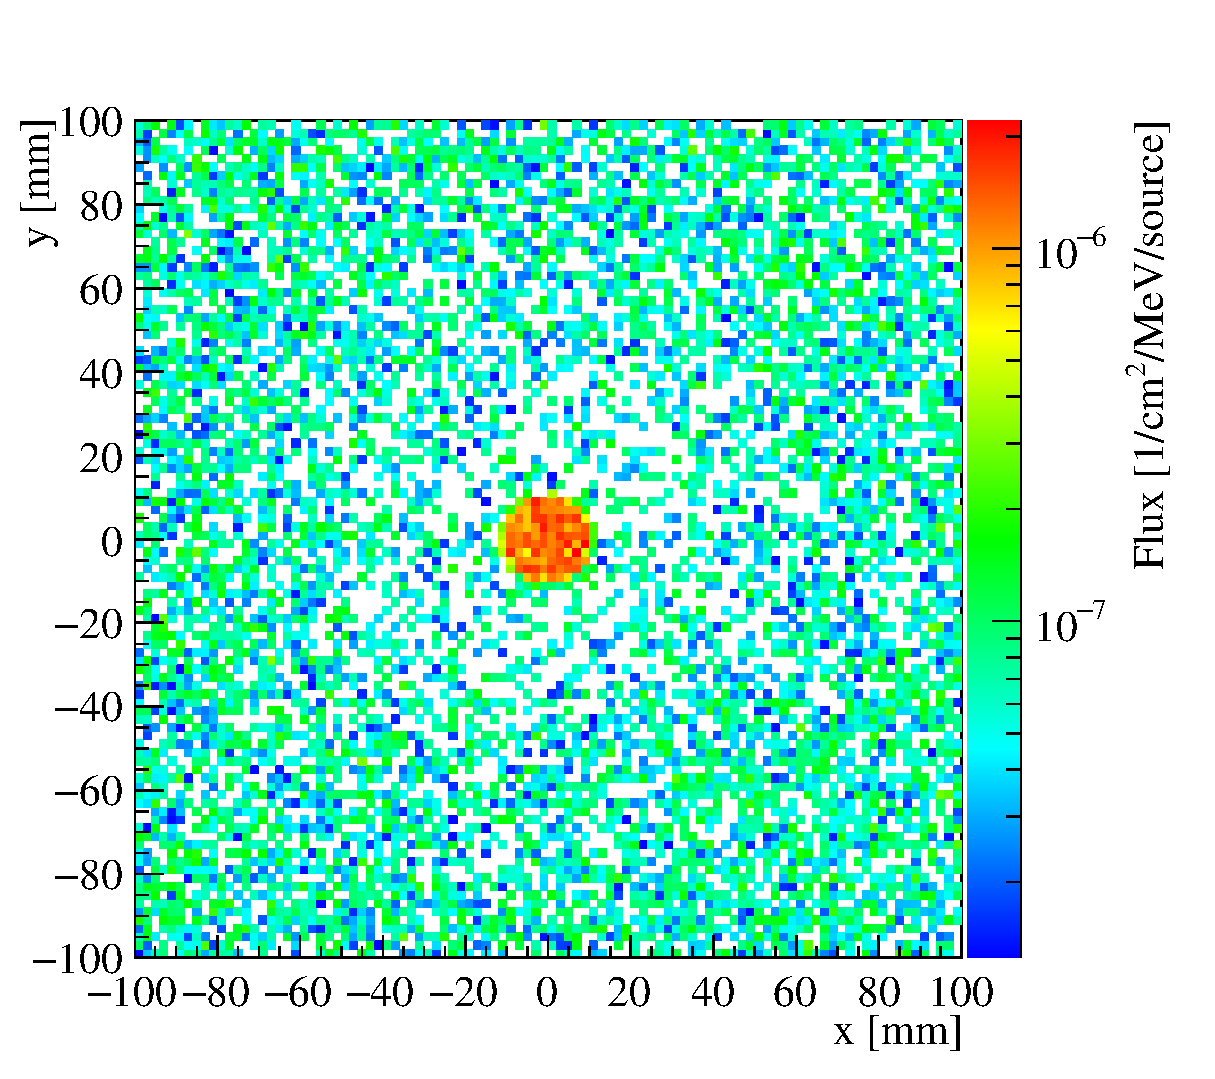
\includegraphics[clip, width=\columnwidth]{cross_xy_f_w_B.eps}
    \caption{ホウ素入りポリエチレンの場合.}
  \end{subfigure}
  \caption{コリメータ通過後の中性子の位置分布.}
  \label{collimator_xy_pos}
\end{figure}
\begin{figure}
  \centering
  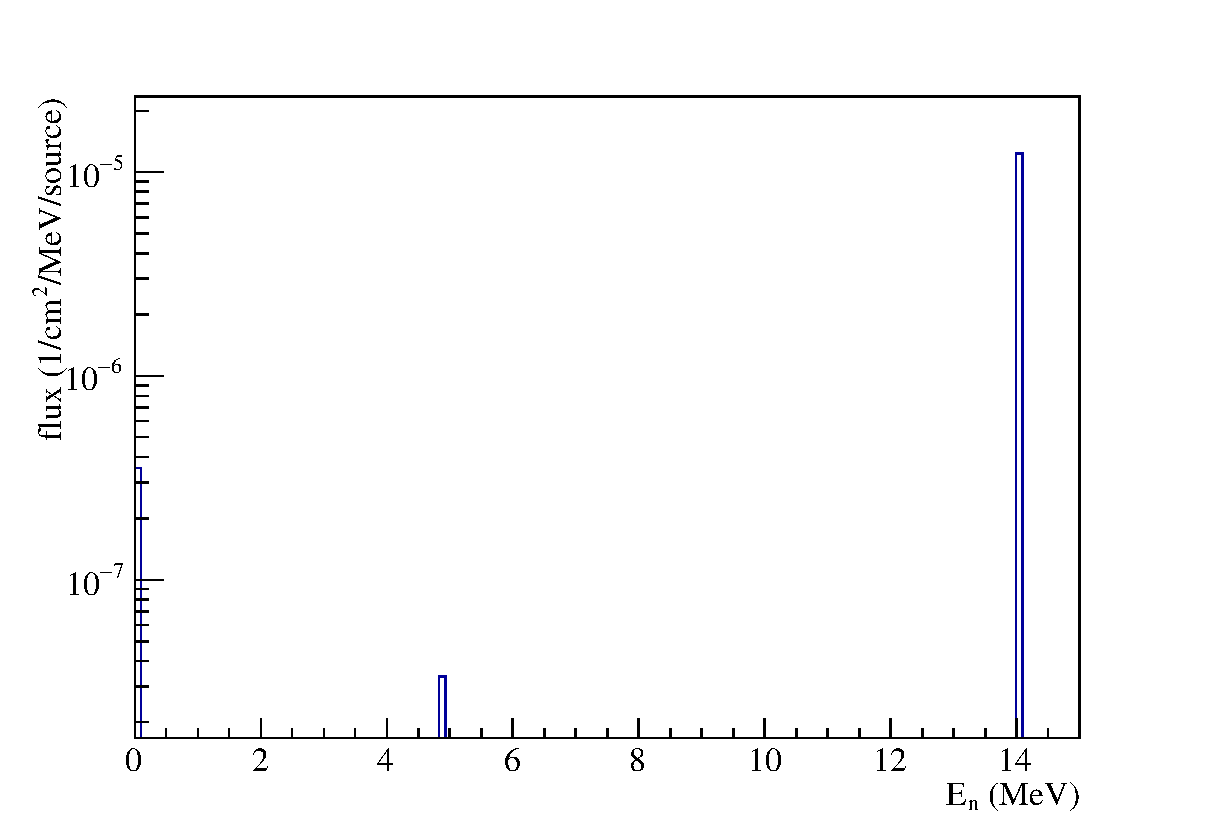
\includegraphics[clip, width=0.8\columnwidth]{cross_eng_f.eps}
  \caption{ポリエチレンコリメータの場合のエネルギー分布.}
  \label{fig::neutron_energy_dist}
  \centering
  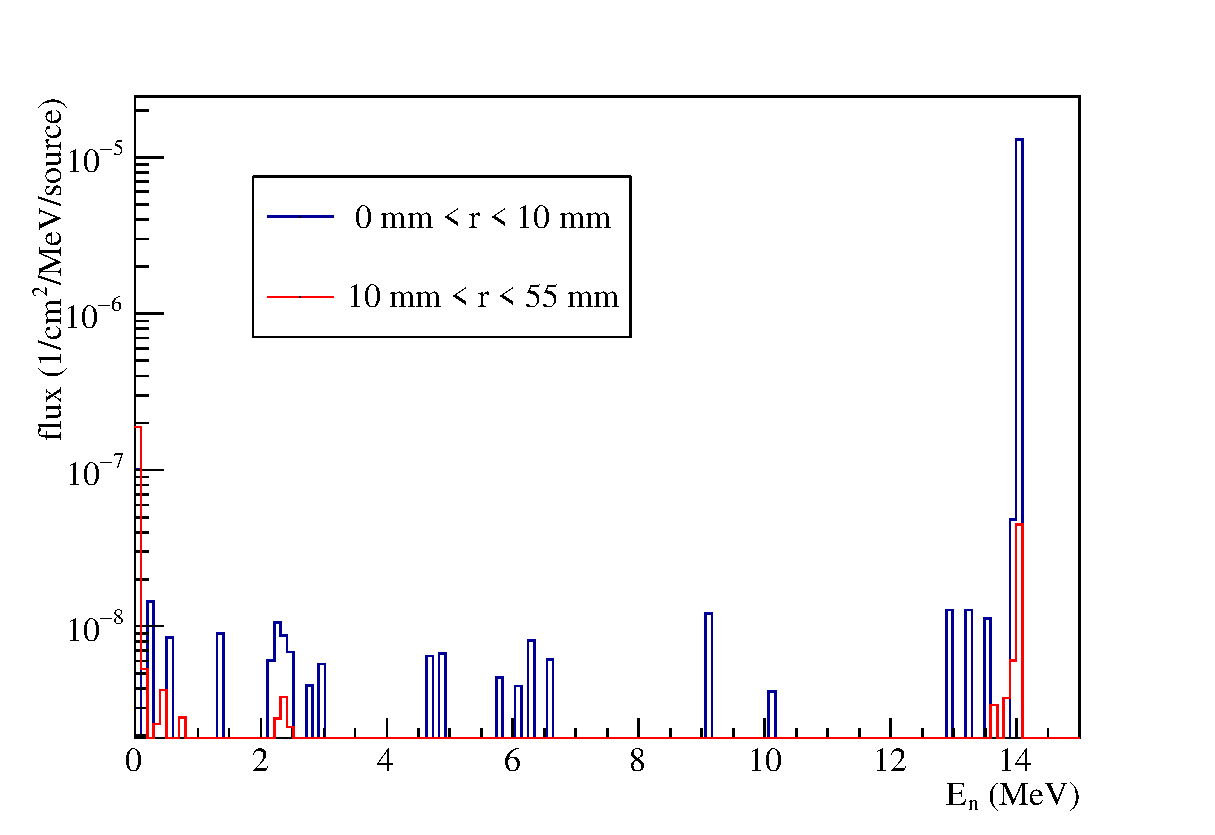
\includegraphics[clip, width=0.8\columnwidth]{cross_eng_f_w_B.eps}
  \caption{ホウ素入りポリエチレンコリメータの場合のエネルギー分布.}
  \label{fig::neutron_energy_dist_w_B}
\end{figure}
\begin{figure}
  \centering
  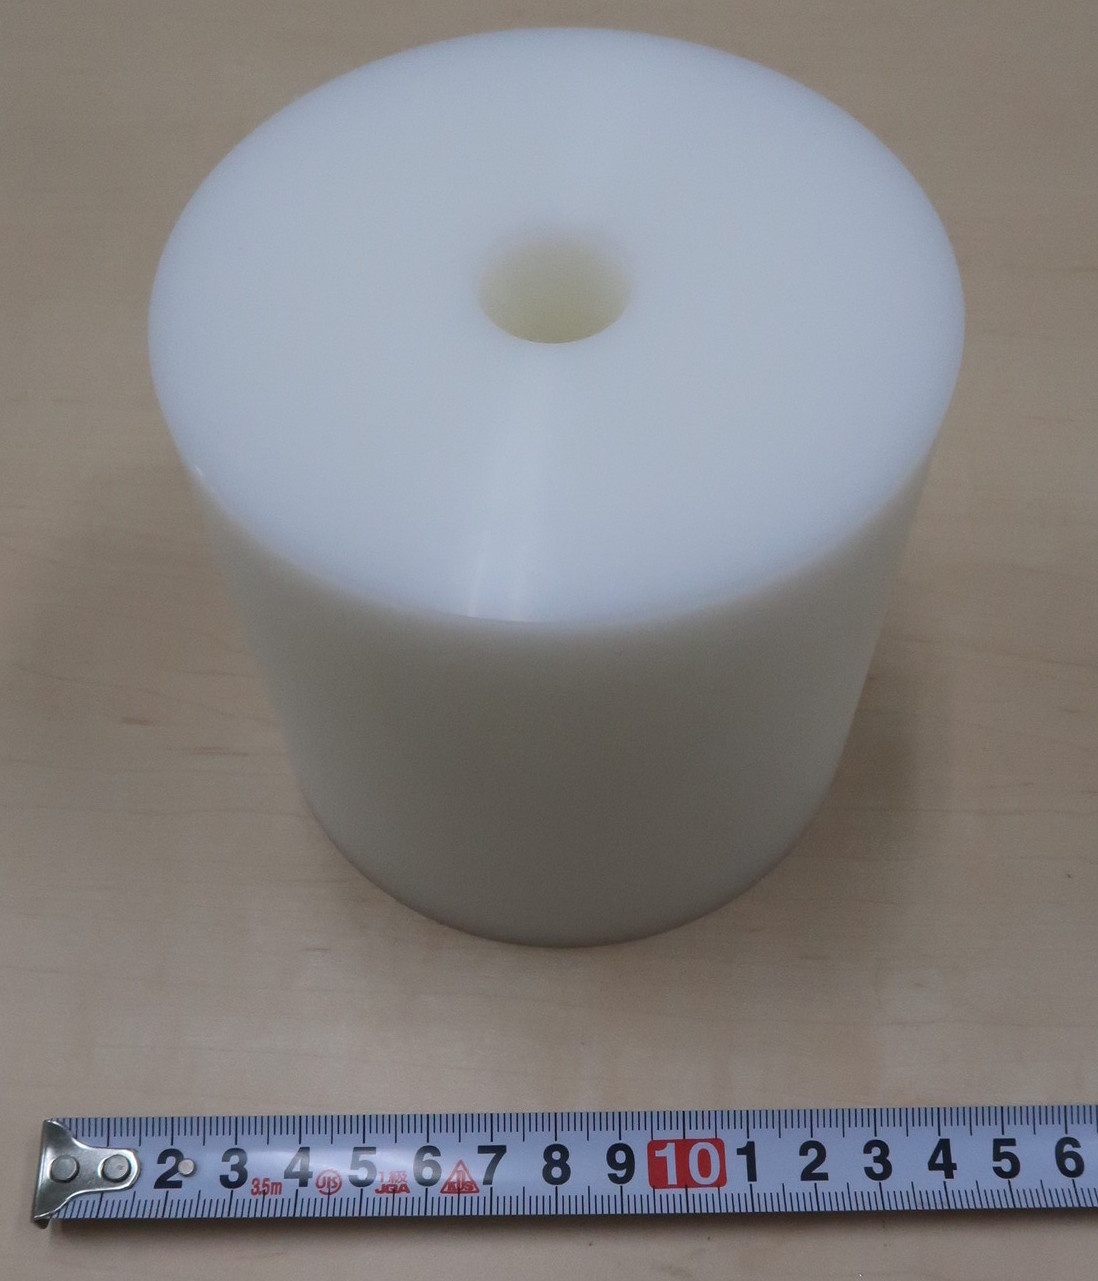
\includegraphics[clip, width=0.8\columnwidth]{IMG_2755_clpd.jpg}
  \caption{ポリエチレンで作成したコリメータ.}
  \label{pic::collimator}
\end{figure}

%\SI{14}{\mega\electronvolt}の中性子は単色エネルギーであることが大きな利点である.
%しかし,コリメータとの散乱によってエネルギーが減少した中性子が入射することが懸念される.
%図\ref{fig::neutron_energy_dist}において,コリメータの中心から\SI{10}{\milli\metre}以内の
%中性子のエネルギーが\SI{14}{\mega\electronvolt}からほぼ変化がないことが分かる.
%よって,中性子のエネルギーが汚れないとして測定を行う.
%\begin{figure}
%  \centering
%  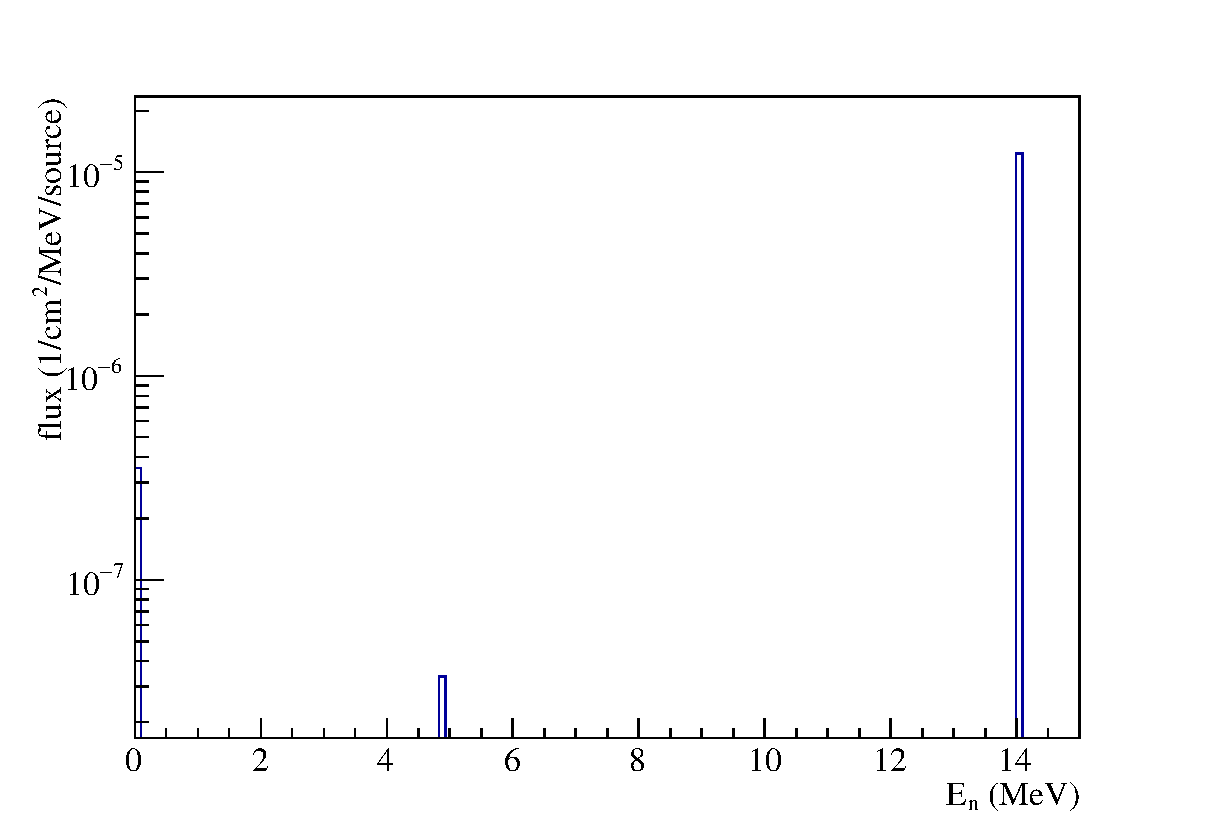
\includegraphics[clip,width=0.8\columnwidth]{cross_eng_f.eps}
%  \caption{コリメータ通過後の中性子のエネルギー}
%  \label{fig::neutron_energy_dist}
%\end{figure}

\section{中性子の収量}
PHITS による計算では\SIrange{0}{10}{\milli\metre}の範囲の
\SIrange{13.9}{14.1}{\mega\electronvolt}の中性子は
\SI{4.07e-5}{\per\mega\electronvolt\per source}となる.
OKTAVIAN のDCビームラインで生成される中性子が\SI{5e9}{\per\second}であるとすると,
コリメータを通過してくる中性子の収量は\SI{4.07e4}{\per\second}となる.

\section{PHITS のインプットファイル}
PHITS のインプットファイルを以下に示す.
ポリエチレンのコリメータの場合のシミュレーションである.
\newpage
\begin{quote}
  \setlength{\baselineskip}{12pt}
\begin{verbatim}
[ T i t l e ]
simulation for neutron collimator

[ P a r a m e t e r s ]
 icntl    =  0
 itall    =  1
 maxcas   =  5000000
 maxbch   =  50
 file(6)  =  phits.out

[ S o u r c e ]
  s-type  =   1
    proj  =   neutron
     dir  =   all
      r0  =   0.
      z0  =  -146.4
      z1  =  -146.4
      e0  =   14.

[ M a t e r i a l ]
 mat[1] $ Air
         N 8 O 2
 mat[2] $ Polyethylene
         C 2 H 4
 mat[3] $ Concrete
         O  -0.52  Si -0.325 Ca -0.06
         Na -0.015 Fe -0.04  Al -0.04
 mat[4] $ Acrylic
         C 5 O 2 H 8
 mat[5] $ Methane
         C 1 H 4

[ S u r f a c e ]
$ colimator
 100   cz   5.5
 101   cz   1.
 102   pz   0.
 103   pz   100.
$ wall
 104   rpp  -100. 100. -100. 100. 0. 100.
$ frange
 110   cz   5.5
 111   pz   102.
 112   pz   104.
$ detector
 120   pz   110.
$ room
 200   rpp  -100. 100. -100. 100. -200. 300.

[ C e l l ]
$ collimator
 100   2   -0.9  -100 +101 +102 -103
$ wall
 200   3   -2.5     -104 +100
$ frange
 300   4   -1.18    -110 +111 -112
$ detector
 400   5   -0.000717 -110 +112 -120
$ room
 1000  1   -0.0012  -200 #100 #200 #300 #400
$ void
 2000  -1           +200

[ T - C r o s s ]
    title =   Energy distribution in r-z mesh (front)
     mesh =   r-z
   r-type =   1
       nr =   3
              0. 1. 5.5 10
   z-type =   1
       nz =   0
              102.
   e-type =   2
       ne =   150
     emin =   0.
     emax =   15.
     unit =   2 
     axis =   eng
     file =   cross_eng_f.out
   output =   f-curr
     part =   all neutron
    gshow =   1
   epsout =   1

[ T - C r o s s ]
    title =   Energy distribution in r-z mesh (rear)
     mesh =   r-z
   r-type =   1
       nr =   2
              0. 1. 5.5
   z-type =   1
       nz =   0
              104.
   e-type =   1
       ne =   3
              0. 13.5 14.5 20.
     unit =   2 
     axis =   eng
     file =   cross_eng_r.out
   output =   f-curr
     part =   all neutron
    gshow =   1
   epsout =   1

[ T - C r o s s ]
    title =   Posion distribution in xyz mesh (front)
     mesh =   xyz
   x-type =   2
       nx =   100
     xmin =  -10.
     xmax =   10.
   y-type =   2
       ny =   100
     ymin =  -10.
     ymax =   10.
   z-type =   1
       nz =   0
              102.
   e-type =   2
       ne =   1
     emin =   0.
     emax =   20.
     unit =   1 
     axis =   xy
     file =   cross_xy_f.out
   output =   f-curr
     part =   all neutron
    gshow =   1
   epsout =   1

[ T - C r o s s ]
    title =   Posion distribution in xyz mesh (rear)
     mesh =   xyz
   x-type =   2
       nx =   100
     xmin =  -10.
     xmax =   10.
   y-type =   2
       ny =   100
     ymin =  -10.
     ymax =   10.
   z-type =   1
       nz =   0
              104.
   e-type =   2
       ne =   1
     emin =   0.
     emax =   20.
     unit =   1 
     axis =   xy
     file =   cross_xy_r.out
   output =   f-curr
     part =   all neutron
    gshow =   1
   epsout =   1

[ T - 3 D s h o w ]
   output =   3
 material = 4
            2 3 4 5
       x0 =   0.
       y0 =   0.
       z0 =   0.
    e-the =   40.
    e-phi =   45.
    e-dst =   500.
    l-the =   150.
    l-phi =   30.
    l-dst =   80.
    w-wdt =   80.
    w-hgt =   100.
    w-dst =   300.
   heaven =   x
     line =   2
   shadow =   2
    resol =   2
     file =   3dshow.out
    title =   Check geometry
   epsout =   1

[Mat Name Color]
  mat    name          color
  1      Air           pastelblue
  2      Polyethylene  red#yellow
  3      Concrete      camel
  4      Acrylic       blue

[ E n d ]
\end{verbatim}
\end{quote}

\end{document}
